\cardfrontfoot{Kapitel 14}
\begin{flashcard}[Egenskab]{Opskriv 3 ioniske, 2 covalente og 2 metalliske carbider}
Ioniske: \ce{Na2C2}, \ce{Be2C} og \ce{Al4C3}\\ \vspace{7pt}
Covalente: \ce{SiC} og \ce{B4C}\\ \vspace{7pt}
Metalliske: \ce{WC} og \ce{Fe3C}
\end{flashcard}

\begin{flashcard}[Anvendelse]{Angiv en anvendelse af \ce{Na2C2}}
\ce{Na2C2 + 2H2O -> 2NaOH + C2H2}
\end{flashcard}

\begin{flashcard}[Fremstilling]{Angiv med reaktionsskema en metode til at fremstille carbonmonoxid i laboratoriet}
\ce{HCOOH + H2SO4(l) -> CO + H2O + H2SO4(aq)}
\end{flashcard}

\begin{flashcard}[Fremstilling]{Angiv med reaktionsskema hvordan man kan fremstille methanol og propanal ud fra bl.a. carbonmonoxid}
\ce{CO + 2H2 -> CH3OH} \\ \vspace{7pt}
\ce{CO + C2H4 + H2 -> C2H5CHO}
\end{flashcard}

\begin{flashcard}[Anvendelse]{Hvordan kan man undersøge om der er carbondioxid i en gasstrøm?}
Man kan lede strømmen gennem en opløsning af  \ce{Ba(OH)2} eller \ce{Ca(OH)2}. Testen er positiv hvis der opstår et bundfald.
\end{flashcard}

\begin{flashcard}[Reaktion]{Beskriv med reaktionsskema hvad der sker når man varmer følgende faste carbonater op:\\ \vspace{7pt}
\ce{CaCO3}, \ce{Ag2CO3}, \ce{(NH4)2CO3} og \ce{NaHCO3}
}
\ce{CaCO3 ->[\text{$\Delta$}] CaO + CO2}\\ \vspace{7pt}
\ce{Ag2CO3 ->[\text{$\Delta$}] Ag2O + CO2}\\
\ce{Ag2O ->[\text{$\Delta$}] 2Ag + $\frac{1}{2}$O2}\\ \vspace{7pt}
\ce{(NH4)2CO3 ->[\text{$\Delta$}] 2NH3 + H2O + CO2}\\ \vspace{7pt}
\ce{2NaHCO3 ->[\text{$\Delta$}] Na2CO3 + H2O + CO2}
\end{flashcard}

\begin{flashcard}[Fremstilling]{Beskriv med reaktionsskema hvordan man fremstiller carbondisulfid industrielt}
\ce{CH4 + 4S(l) ->[\text{$\Delta$}] CS2 + 2H2S}
\end{flashcard}

\begin{flashcard}[Fremstilling]{Opskriv to metoder til at producere \ce{CCl4}}
\begin{itemize}
\item \ce{CS2 + 3Cl2 ->[\text{$\rm FeCl_{3}/\Delta$}] CCl4 + S2Cl2}\\
\ce{CS2 + 2S2Cl2 ->[\text{$\Delta$}] CCl4 + 6S}
\item \ce{CH4 + 4Cl2 -> CCl4 + 4HCl}
 \end{itemize}
\end{flashcard}

\begin{flashcard}[Fremstilling]{Angiv to industrielle metoder til at fremstille blåsyre}
\ce{CH4 + NH3 ->[\text{$\rm Pt/1200\,^{\circ}{\rm C}$}] HCN + 3H2}\\ \vspace{7pt}
\ce{2CH4 + 2NH3 + 3O2 ->[\text{$\rm Pt/Rh/1100\,^{\circ}{\rm C}$}] 2HCN + 6H2O}
\end{flashcard}

\begin{flashcard}[Fremstilling]{Opskriv hvordan man fremstiller silicium industrielt}
\ce{SiO2 + 2C ->[\text{$\Delta$}] Si(l) + 2CO}
\end{flashcard}

\begin{flashcard}[Fremstilling]{Opskriv to metoder til at oprense silicium industrielt}
Følgende ligevægt kan bruges til at destillere silicium. Ligevægten er forskudt med højre ved ca $300\,^{\circ}{\rm C}$ og mod venstre ved $1000\,^{\circ}{\rm C}$.\\
\ce{Si + 3HCl <=> SiHCl3(g) + H2}\\ \vspace{7pt}
En alternativ metode er zone-refining:
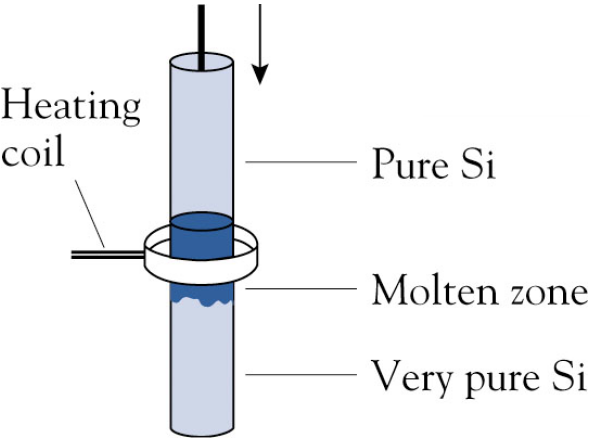
\includegraphics[width=0.37\textwidth]{figures/k14s340ZoneRefining.png}
\end{flashcard}

\begin{flashcard}[Reaktion]{Opskriv den kemiske formel for to kemikalier som kan reagere med glas samt deres reaktion}
Der er tale om \ce{HF} og \ce{NaOH}\\ \vspace{7pt}
\ce{SiO2 + 6HF -> SiF6^{2-} + 2H+ + 2H2O}\\ \vspace{7pt}
\ce{SiO2 + 2NaOH ->[\text{$\Delta$}] Na2SiO3 + H2O}
\end{flashcard}

\begin{flashcard}[Egenskab]{Opskriv de fire typer glas der er omtalt i bogen og angiv fordele ved hver af dem}
\begin{itemize}
\item Soda-lime\\Billigt
\item Borosilicate\\Kan klare store temperaturudsving
\item Lead\\Absorberer radioaktiv stråling
\item Quartz\\Er også gennemsigtigt i UV området
\end{itemize}
\end{flashcard}

\begin{flashcard}[Fremstilling]{Angiv med reaktionsskema hvordan man kan fremstille natriumsilicat}
\ce{SiO2 + 2Na2CO3(l) ->[\text{$\Delta$}] Na4SiO4 + 2CO2}
\end{flashcard}

\begin{flashcard}[Struktur]{Tegn strukturen af pyrosilicationen}
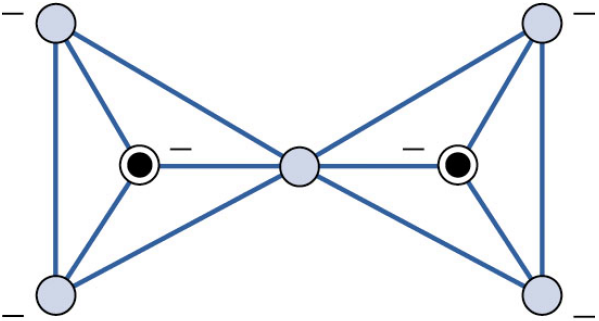
\includegraphics[width=0.5\textwidth]{figures/k14s344Pyrosilicate.png}
\end{flashcard}

\begin{flashcard}[Reaktion]{Angiv reaktionen mellem silicationen og syre}
\ce{2SiO4^{4-} + 2H+ -> Si2O7^{6-} + H2O}
\end{flashcard}

\begin{flashcard}[Struktur]{Angiv de kemiske formler for hvid og blå asbest og angiv hvilken der er farligst}
Hvid asbest: \ce{Mg3(Si2O5)(OH)4}\\ \vspace{7pt}

Blå asbest: \ce{Na2Fe5(Si4O11)2(OH)2} (farligst)
\end{flashcard}

\begin{flashcard}[Fremstilling]{Angiv hvordan silikone laves ved hjælp af reaktionsskemaer samt strukturen af silikone}
\ce{2CH3Cl + Si ->[\text{$\Delta$}] (CH3)2SiCl2}\\
\ce{(CH3)2SiCl2 + 2H2O -> (CH3)2(Si(OH)2 + 2HCl}\\
\ce{$n$(CH3)2Si(OH)2 -> [-O-Si(CH3)2-]_{$n$} + H2O}\\ \vspace{7pt}
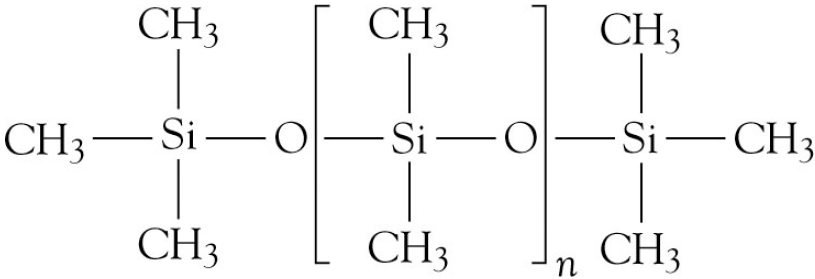
\includegraphics[width=0.9\textwidth]{figures/k14s349Silikone.png}
\end{flashcard}

\begin{flashcard}[Reaktion]{Angiv tin(II)oxids reaktion med syre henholdsvis base}
\ce{SnO + 2HCl -> SnCl2 + H2O}\\ \vspace{7pt}
\ce{SnO + NaOH + H2O -> Na+ + [Sn(OH)3]-}
\end{flashcard}

\begin{flashcard}[Fremstilling]{Angiv den primære kilde af bly i naturen samt hvordan man udvinder bly fra denne}
Den primære naturlige kilde er \ce{PbS}\\ \vspace{7pt}
\ce{2PbS + 3O2 ->[\text{$\Delta$}] 2PbO + 2SO2}\\
\ce{PbO + C ->[\text{$\Delta$}] Pb + CO}
\end{flashcard}

\begin{flashcard}[Reaktion]{Angiv med reaktionsskema hvorledes \ce{PbCl4} dekomponerer}
\begin{align*}
\ce{\OX{rf1,\ox{+4,\ce{Pb}}}\OX{of1,\ox{-1,\ce{Cl4}}} -> \OX{re1,\ox{2,\ce{Pb}}} Cl2 + \OX{oe1,\ox{0,\ce{Cl2}}}}
\redox(of1,oe1){\small oxidation}
\redox(rf1,re1)[][-1]{\small reduktion}
\end{align*}
\end{flashcard}